\section{Biological Regulation}
\label{sec:bioreg}
Information, \ie negative entropy, is present throughout the cosmos at every orders of magnitude, and as its inhabitants, informatavores are witness among many of its scales. The most fundamental operating unit of information processing yet uncovered in biological systems are the RNA and DNA molecules. Reading the molecules which string together to form chains, these mega-molecules confer schematic formulations to the functional units of life, proteins. The mechanisms by which these instructions are read, \ie their order, duration, frequency etc., are a major component of modern biological investigation. Together, these procedural tendencies have developed under many \emph{goldilocks} conditions in a random manner, perhaps directed only through the goal of perpetual negative entropy degradation. To tackle this goal with the highest likelihood of success, these regulatory relationships developed to enable response to any existing stimuli yet encountered. Less frequently and by luck some individuals deviated to account for stimuli which had not yet come to pass but which could. Like evaluating and recalculating for each hand at a blackjack table in order of their probability in accordance to cards already at play, the ability to continue processing negative entropy is ensured by nondeterministically betting on what has been, what is and what could be. Such is the ''safety in numbers'' paradigm, wherein chances of individual survival are overlooked in the context of group persistence, which is a good trade-off for the universe in terms of its goal of completely degrading negative entropy.

Generally speaking, evolution by way of natural selection is a major mechanism of persistent life, breathing forth a continuum of hierarchies from the combination of time and the fundamental forces of and principles driving nature. Building functional relationship among these \emph{endless forms most beautiful and most wonderful}\citep{darwin1869origin}, natural evolution has birthed a level of information storage and processing in the form of living organisms. In the right setting, the DNA molecule allows for not only the high fidelity storage of any set of biological blueprints (partially through its own replication), but the generation of various forms of more pliable, actionable RNA molecules to carry out its will. In unison with post-translational factors, transporters, etc., these various RNA molecules dictate the expression of proteins which carry out the life process, including all mechanisms of storing, reading and repairing progenitor molecules. Regulation of influence and oversight whereby one or more molecules (directly or indirectly) dictate the behavior of another surely developed concurrently, growing in complexity as information storage and retrieval became more reliable and expansive, allowing for more creative and elaborate solutions to most natural environment yet exposed to life. Looking at such complexity without the aid of the very time it took to develop each sequential development has only recently become a tractable problem interpretable through the modern hominid alliance with outboard processors.

Science has long sought to understand the regulatory mechanisms guiding living bodies. Past attempts have placed constraints on possible regulatory capabilities, however many have since been overturn or amended through further, quasi-\emph{post-modern} study (famously the popular interpretation of Crick's central dogma \cite{crick1958protein}). In the light of such overturned or amended dogma, any similarly bold claim seems n\"{a}ive in the extreme. Today it is understood that bodies are composed of proteins whom act in concert with not only those constituents, but with its surrounding environment. Crucially, proteins have come upon a means to affect change in other proteins behavior largely through binding, \eg regulating expression or enzymatic activity, which can be used to develop the array of living functions, such as building ion gradients along a membrane in the protein's environment. Regulation of these highly flexible, redundant and robust systems comes down to cause and effect, \ie one player dictating the behavior of another; but do not think this discourse ends so cleanly. When mapped these regulations are hairball-like \cite{schulz2013grooming}, seemingly departing from each node while also arriving at every other node (an unlikely biological prospect). In the specific domain of gene regulation explored here, this entails the regulation of a gene's transcription by the aptly named transcription factor (TF). This regulation varies in how much any given gene's product is expressed by the various cellular machinery as an RNA molecule on its way to be separately regulated, processed and translated into a protein. Whether investigating proliferation of cell subtypes within a heterogeneous cancer mass or the tumbling quorum sensing of bacterial flagella used to seek out environments advantageous to its energy cycle, reliable roads of communication among machinery are crucial to continued survival.

Gene expression is dictated at the level of transcription through the physical binding of a TF upstream from a gene's start codon (any nucleotide (alphabet of DNA) triplet, \cref{fig:DNA}) which is then likely to be translated to RNA for processing to actionable protein. These TF binding relationships are often highly specific, but because of robust functionality can also be somewhat promiscuous, regulating multiple genes whose products act in unison toward some complimentary function or completely independent. Since TF are nothing more than proteins themselves, the protein product of any regulated gene can then itself play a regulatory role on any number of other genes (notice the overall cyclic nature of \cref{fig:DNA}). Hence the problem evolves from one of strictly direct relations to include those secondary, etc. indirect relations, begetting the hairball of interactions which govern the life process. The question may arise to the fitness advantage of redundant pathways to carry out similar functionality, and this is where one must consider speed to functionality over time. Delayed onset of function can prepare secondary responses to environmental assaults, among other capabilities, and so while the end goal of pathways may look identical in hindsight, details of the cell's present may necessitate the subtle variation in when the response is brought into play. So crucial are these relationships to the wild-type functioning of any cell, however, as is to be expected, when operating over many independent variables, direct relationships are often muddling and ambiguous. Creating ordered, predictable responses to internal and external stimuli is at the heart of the life process, and these are precisely what we mean to uncover.

%%mention next gen seq: ion/454-pyro (SU)/sanger/illumina/solid
Several methods are available for quantifying and characterizing biology to allow resolution of regulatory machinery through perturbation-based network inference, and generally include but are not limited to microarray, qPCR, RNA-Seq/ transcriptome methods and finally survival/phenotypic assay. As with all developing technologies there are trade-offs in what specifically is under investigation, and what can be overlooked to afford that focus. As may be expected, these various techniques are positioned with advantage to certain levels of biology and their collective characterizations are thus segregated and gathered in (often isolated) databases. Known interactions are very similarly cataloged, where known TF binding interactions in the model organism \emph{E.coli} are housed in \emph{RegulonDB}\cite{gama2008regulondb}, while \emph{Yeastract}\cite{teixeira2006yeastract} houses those for \emph{S.cerevisiea}. These are quite useful when gold standards are sought to check against networks inferred from new platforms, to validate findings and classify possible novel interactions (say as stemming from known hub genes, etc.).

\begin{figure}%[H]
\centering
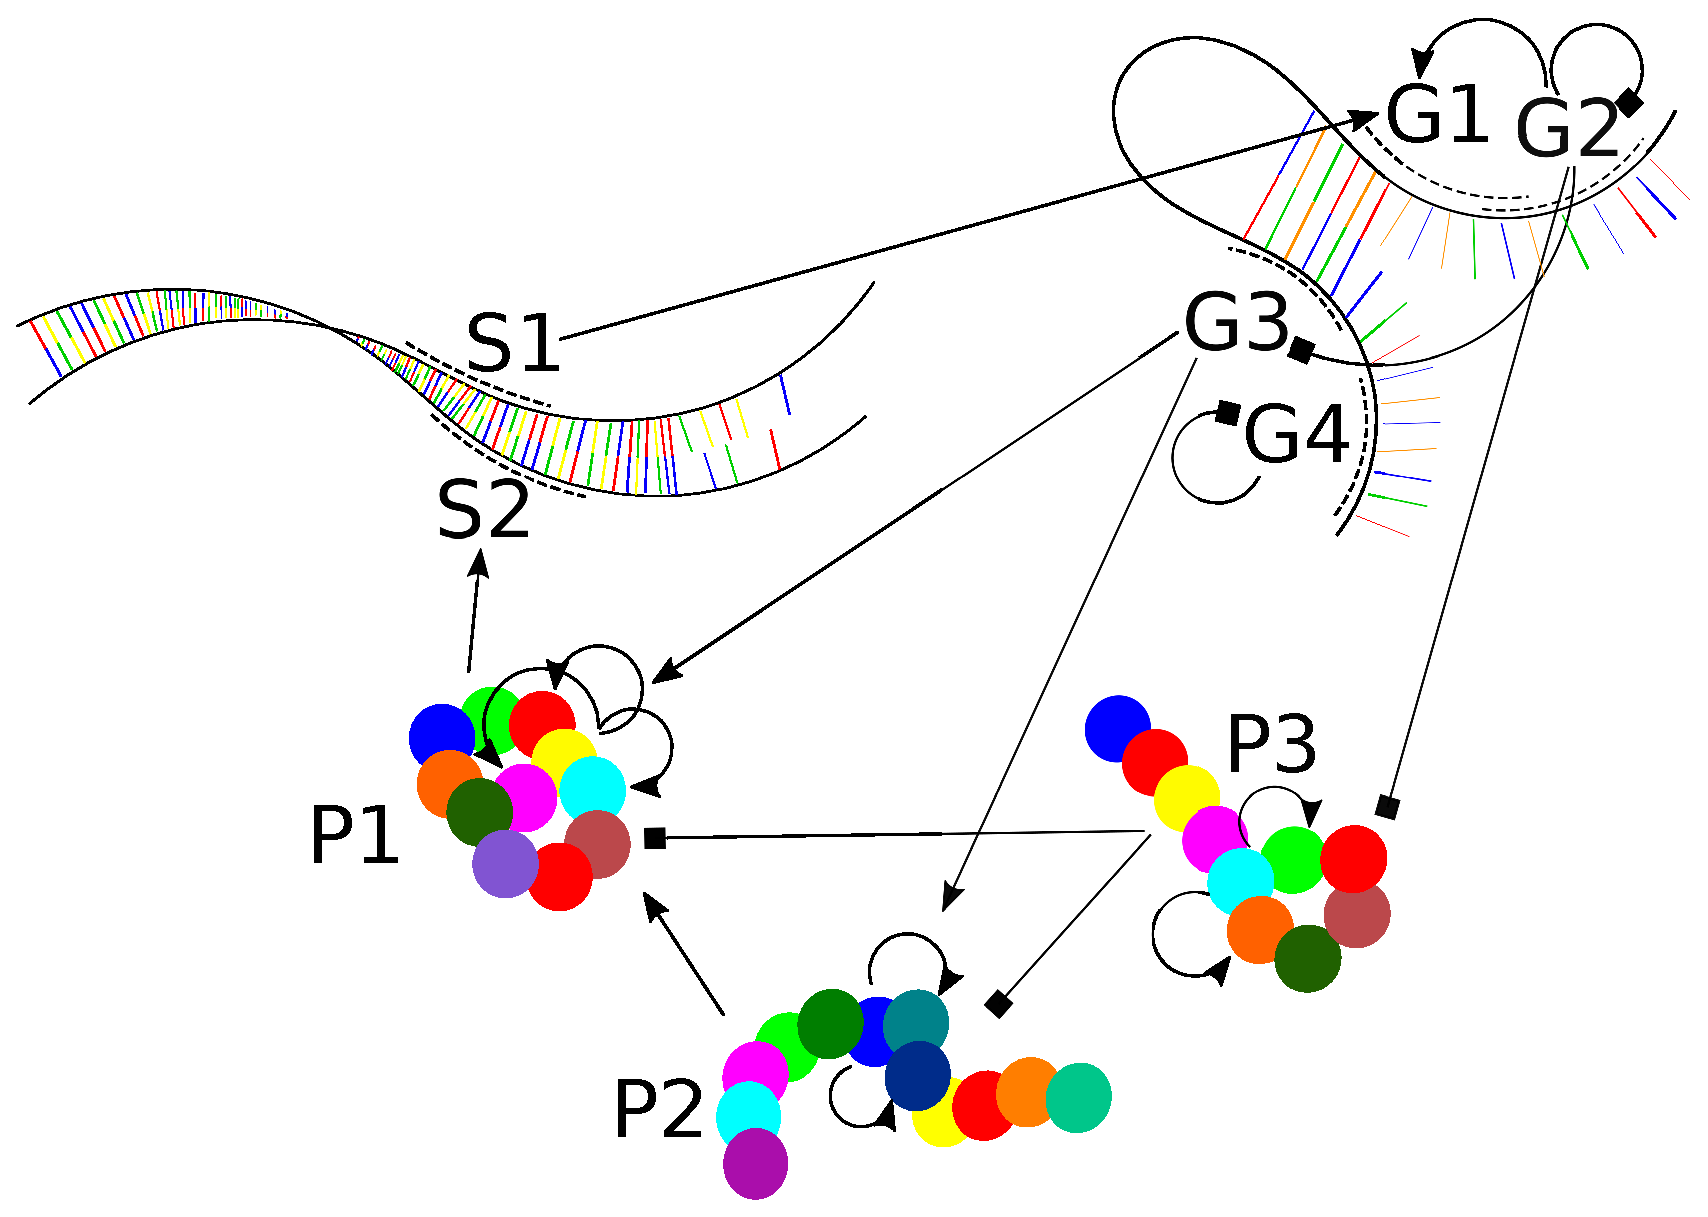
\includegraphics[width=1\linewidth]{2/DNA2.eps}
\caption{{\textbf Agnostic Biological Regulation.} Elements are seen to regulate one another regardless of biological mode/level, leading to loops as well as cascades of regulatory signaling. The regulation need not be direct, as this example contains no two factors directly linked but rather factors are linked between both the three distinct biological levels of DNA Sequence (S), RNA Gene (G) and Protein (P) as well as within level, /ie G2->G1, P3->P2->P1. In this example, S1 upregulates G1, which itself is also upregulated by G2, which concomitantly down-regulates G3 and P3. P3 would normally directly bind and  both P1 and P2, however the partial absence of both now limit upregulating expression of S2 to initiate further regulation (not shown).
}
\label{fig:DNA}
\end{figure}


\subsection{Implication}
\label{sec:practical}
A better understanding of the interplay between constituent regulators throughout every level of biology is crucial toward the development of any form of personalized or precision medicine \citep{barabasi2011network}. A recent study linked a large portion of human genes, some 17000 to over 15000 diseases, disorders or abnormal phenotypes \citep{pinero2015disgenet}, making for nearly half a million unique gene-disease associations. Only by placing these components together can we glean practical insights towards actionable intervention in the general systemic decay leading to disease onset, development and progression. Genotyping of certain disease markers simplifies the search-space in individual patients, making it possible to give reasonable developmental predictions, many of which have actionable responses to prevent any (further) future damage to the patient, \ie BRCA1 \citep{lerman1996brca1}. Such relationships are continually uncovered, revealing more of nature's order, enabling, for example, ever wider fetal defect screening for expectant mothers, \ie heart defects \citep{hyett1999using} as well as for those in especially compromising climates around the world vulnerable to certain debilitating disease.

In addition to identifying biomarkers, such GRN can draw upon knowledge describing disease in other contexts, ie correlating certain SNPs, a resource bloating databases but seldom used to describe systems, to complex traits \cite{platig2016bipartite}. In this way databases become enriched with new regulatory knowledge, expanding use for SNP and other such isolated data for use by the community and more simply profiling new patients, expanding the use of SNP profiling, for example.

Drug development is another area with huge interest in the interaction among biomolecules. By understanding the relationships present in a individual and tracking them as they change during disease development one can uncover exact targets for drug intervention. It is not so simple to say once a target is known a treatment can be found, but it is a stronger point of development than has widely been available before. What is more promising is the targeting of gene modules, complexes or regulatory subnetworks so interdependent that knocking out one element alters the activity of the rest, thus offering a nevertheless real means of affecting change in patients. A growing field and a personal ambition lies in the use of, among other approaches, directed acyclic graphs (DAGs) or networks /GRNto screen profiles of compounds, to repurpose adverse side effects to affect change in disparate classes of patients. The more completely this interactive landscape is detailed, the more directly compounds targeting similar combinations of sites in antagonism with disease progression can be identified, not to mention the more powerful but more complex prospect of designing targeting molecules. Whether by repurposing, \ie {repositioning}, drugs tested to be safe for human consumption, or designing new drugs to treat new disease, accurate knowledge of the mechanisms underlying developmental paths toward disease are key, and an aspect of which can be gleaned from reliable network inference approaches.
